\documentclass[10pt,usenames,dvipsnames]{beamer}

\usepackage{amsmath, mathtools, siunitx}
\usepackage[none]{hyphenat} %removes hyphenation at end of lines
\usepackage{caption}
\usepackage{subcaption}
\usepackage{graphics,graphicx,epsfig,ulem, booktabs} % Makes sure all graphics works
\usepackage{amssymb}
\usepackage{float}
\usepackage{multicol, multirow}
\usepackage{enumitem}
\usepackage{color, soul}
\usepackage{gensymb}
\usepackage{sidecap}
\usepackage{cancel}
\usepackage{wrapfig}
\usepackage{xcolor}
\usepackage{pifont}
\setlist[itemize]{noitemsep, topsep=-8pt}
\setlist[enumerate]{topsep=-8pt}
\sidecaptionvpos{figure}{c}

\usetheme{Berkeley}
\usecolortheme{beetle}

\newcommand{\labelitemi}{\color{CadetBlue} \ding{228}}

\title{Quarkonium}
\subtitle{Physics Problem Solving Project}
\author{Matthew Rossetter}
\institute{
    Durham University
}
\date{\today}

\begin{document}

\frame{\titlepage}

\begin{frame}
    \frametitle{Introduction}
\end{frame}

\begin{frame}
    \frametitle{Background}
\end{frame}

\begin{frame}
    \frametitle{Numerical Methods for Solving the Wavefunction}
\end{frame}

\begin{frame}
    \frametitle{The Milestone Project}
    \framesubtitle{Solving the Hydrogen Wavefunction}
    \begin{columns}[c]
        \column{0.5\textwidth}
        \begin{center}
            \includegraphics[scale=0.2]{images/hydro.png}
        \end{center}
        \begin{itemize}
            \item Program for Quarkonium applied to Hydrogen
            \item $\frac{4\alpha_s}{3} \to \frac{1}{137}, \beta \to 0, \mu \to m_e$
            \item Iterate over energies
        \end{itemize}
        \column{0.5\textwidth}
        \begin{itemize}
            \item $E_{1,0} = -13.6\,$eV
            \item $E_{2,0} = -3.39\,$eV
            \item $E_{2,1} = -3.25\,$eV
            \item Energies close to real values
        \end{itemize}
        \begin{center}
            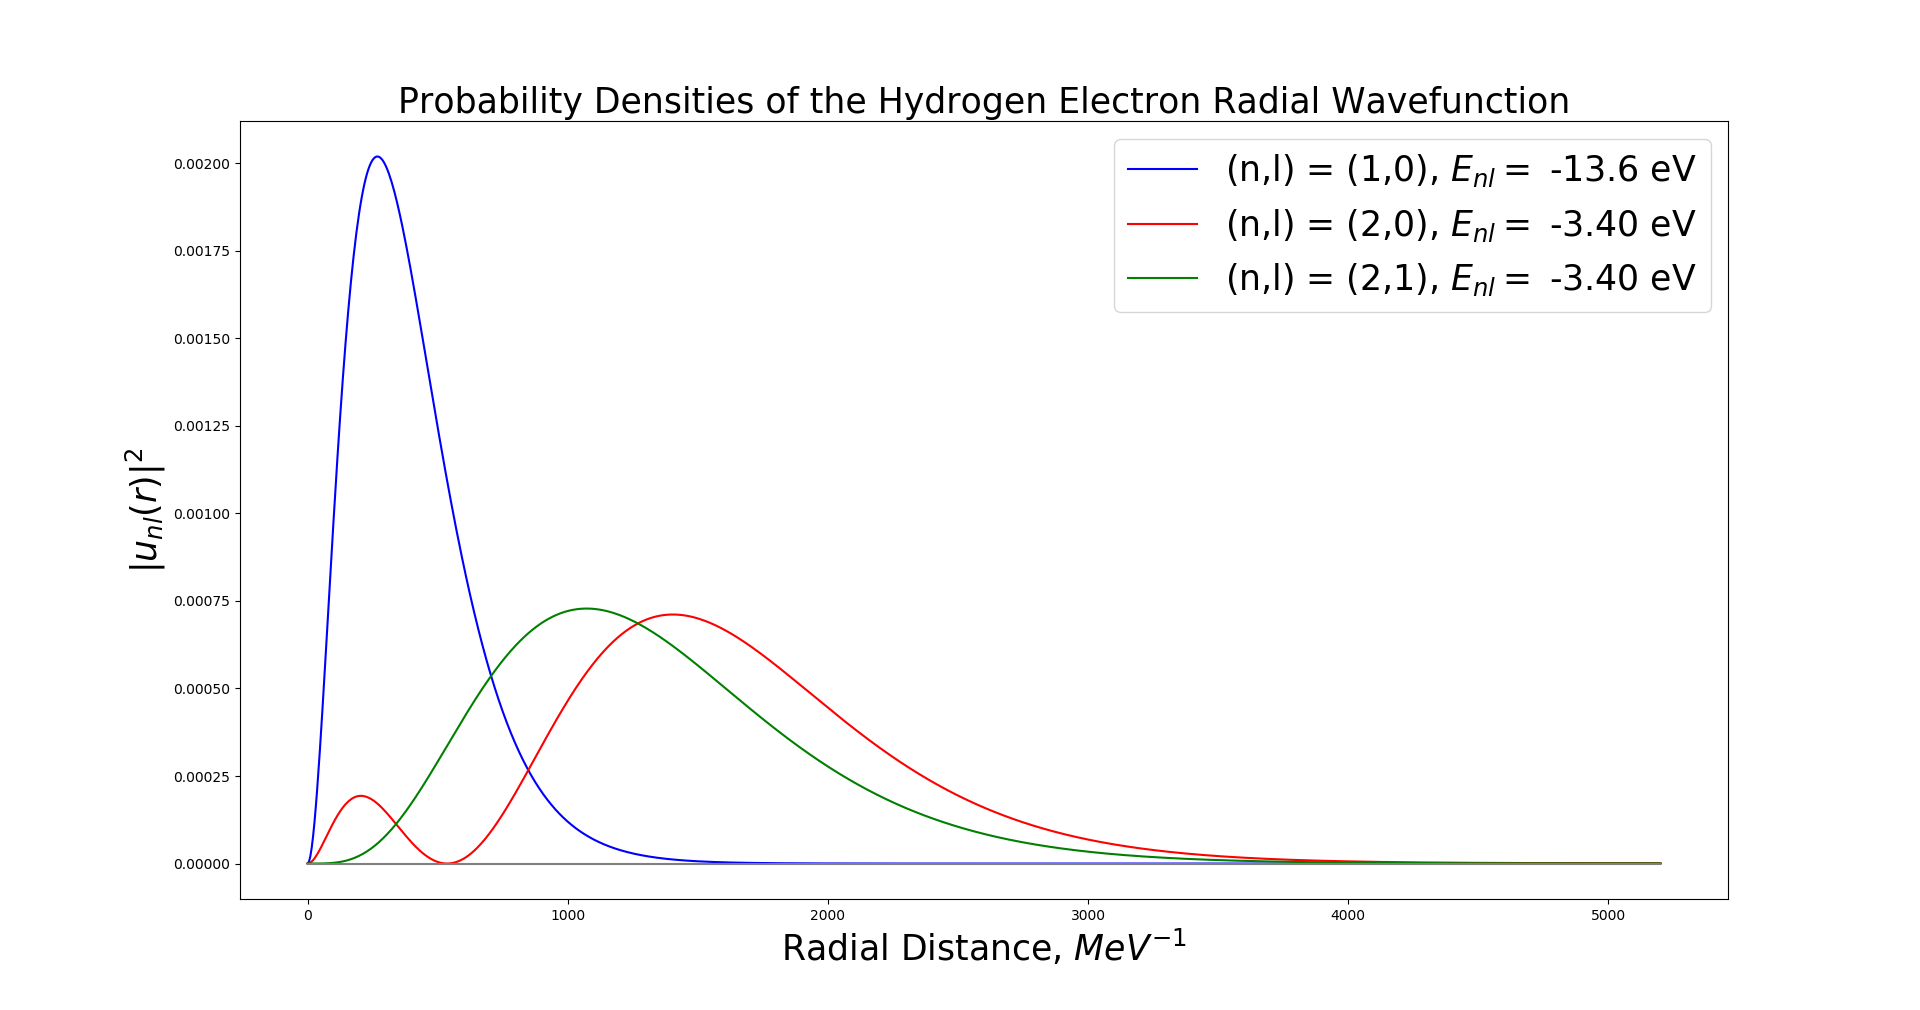
\includegraphics[scale=0.2]{images/probs.png}
        \end{center}
        \end{columns}
\end{frame}

\begin{frame}
    \frametitle{Further Extensions}
\end{frame}

\end{document}
